\documentclass[../document.tex]{subfiles}

\begin{document}
    \subsection{Индивидуальное задание практики}
    \par В качестве индивидуального задания практики было поручено исследовать возможность распознавания медведей при помощи методов машинного обучения.
    \par Само по себе распознавание медведей является актуальной и интересной задачей, так как разработанные решения можно использовать для:
    \begin{itemize}
    	\item Исследование поведения медведей
    	\item Обеспечение безопасного проведения работ в областях, которые расположены в местах обитания медведей
    	\item Исследование миграции медведей
    	\item Наблюдение за медведями в местах их содержания(вольеры, заповедники и т.д.)
    \end{itemize}
    
    \subsection{Выбор моделей}
    \par Для выполнения задания в первую очередь требовалось выбрать рассматриваемые модели. К моделям были применены следующие требования, а именно:
    \begin{itemize}
    	\item Быстродействие
    	\item Точность
    	\item Возможность решать задачи классификации изображений или детекции
    \end{itemize}
    \par В частном случае задача детекции была превращена в задачу классификации, так как если модель смогла на изображении найти объект с нужным классом, то в качестве ответа получали только метку класса, а именно есть медведь на изображении или он отсутствует.
    \par Были выбраны следующие модели:
    \begin{itemize}
    	\item YOLO
    	\item RT-DETR
    	\item Faster R-CNN
    \end{itemize}
    \par Для всех моделей были использованы веса, которые обучили на датасете Common Objects in Context (COCO).
    
    \subsection{YOLO}
    \par Когда в задаче говорится о детекции объектов, то в первую очередь для решения этой задачи в голову приходит архитектура YOLO.
    \par YOLO (You Only Look Once), популярная модель обнаружения объектов и сегментации изображений, была разработана Джозефом Редмоном и Али Фархади в Университете Вашингтона. Появившись в 2015 году, YOLO быстро завоевала популярность благодаря своей высокой скорости и точности.
    \par На сегодняшний день существует не менее 10 версий описываемой архитектуры.
    \par Алгоритм YOLO, был первой попыткой сделать возможной детекцию объектов в реальном времени. В рамках алгоритма YOLO исходное изображение сначала разбивается на сетку из $N×N$ ячеек. Если центр объекта попадает внутрь координат ячейки, то эта ячейка считается ответственной за определение параметров местонахождения объекта. Каждая ячейка описывает несколько вариантов местоположения ограничивающих рамок для одного и того же объекта. Каждый из этих вариантов характеризуется пятью значениями — координатами центра ограничивающей рамки, его шириной и высотой, а также степени уверенности в том, что ограничивающая рамка содержит в себе объект. Также необходимо для каждой пары класса объектов и ячейки определить вероятность того, что ячейка содержит в себе объект этого класса. Таким образом, последний слой сети, принимающий конечное решение об ограничивающих рамках и классификации объектов работает с тензором размерности $N×N×(5B+C)$, где $B$ — количество предсказываемых ограничивающих рамок для ячейки, $C$ — количество классов объектов, определённых изначально.
    
    \begin{figure}[H]
    	\centering
    	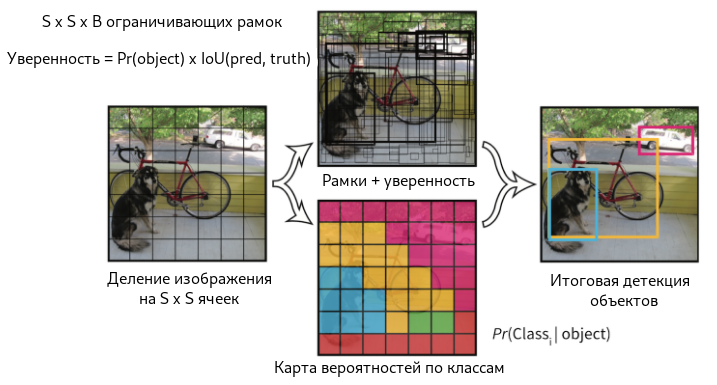
\includegraphics[scale=0.5]{YOLO_alg.png}
    	\caption{Алгоритм YOLO}
    	
    	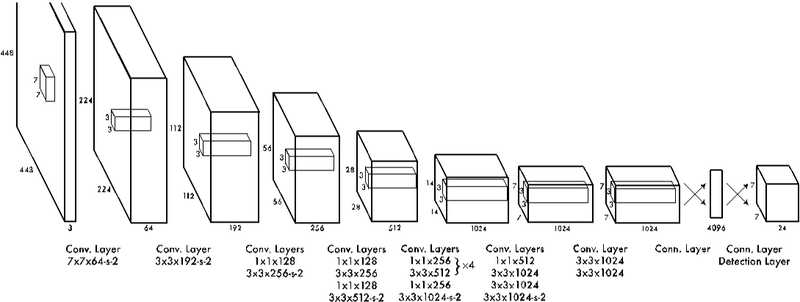
\includegraphics[scale=0.5]{YOLO_arch.png}
    	\caption{Архитектура YOLO}
	\end{figure}
	
	\par какой-то текст для теста
	\par какой-то текст для теста
	\par какой-то текст для теста
\end{document}
